% SC2203 --- Chapter 8: Complexity -- P, NP, NP-Completeness (0->100 ground-up)
\chapter{Complexity: $P$, $NP$ and $NP$-Completeness}
\label{ch:complexity}

\begin{quote}
\emph{``Can we solve it quickly, or only verify quickly?''} --- $P$ vs.\ $NP$ separates feasible from merely checkable; Cook--Levin shows SAT is the hardest checkable problem, and reductions propagate hardness to CLIQUE, 3SAT, and beyond.
\end{quote}

\noindent\fbox{\parbox{\dimexpr\linewidth-2\fboxsep-2\fboxrule}{%
\textbf{From zero: we build here, no complexity assumed.} We define $P$ and $NP$ from scratch---deterministic vs.\ certificate verifiers, time as TM steps---with pictures of exponential vs.\ polynomial growth before formalism. Cook--Levin and SAT$\to$CLIQUE are proved in outline; coping strategies close the book. Only TMs and reductions required.}}
\vspace{0.4em}

\section*{Learning Outcomes}
After this chapter you will be able to:
\begin{enumerate}[label=(L\arabic*)]
    \item define $TIME(t(n))$, $P$, $NP$ via verifiers and via NTMs, and explain the two $NP$ views;
    \item prove $P\subseteq NP$ and know why $P\neq NP$ is open;
    \item state Cook--Levin: SAT is $NP$-complete, with proof idea (tableau);
    \item give a polynomial-time reduction $SAT\le_p 3SAT\le_p CLIQUE$ and verify it;
    \item list coping strategies for $NP$-complete problems (approximation, FPT, heuristics).
\end{enumerate}

% ============================================================
\section{Time Complexity and $P$}
\label{sec:P}
Fix a (deterministic, single-tape) TM $M$. Its \emph{time} $time_M(n)=\max_{|w|=n}$ steps to halt (worst case). $TIME(t(n))=\{L\mid\exists\text{ DTM }M,\;L(M)=L,\;time_M(n)=O(t(n))\}$. Polynomial time is feasible at scale: $n^3$ stays usable when $2^n$ does not.

\begin{definition}[$P$]
$P=\bigcup_{k\ge1}TIME(n^k)$: languages decidable by a DTM in polynomial time (worst case). $P$ is robust: multi-tape $O(t^2)$, encoding changes, etc.\ give polynomials, so $P$ is model-invariant (Church--Turing + polynomial thesis).
\end{definition}

% TikZ 1: polynomial vs exponential growth
\begin{figure}[h]
\centering
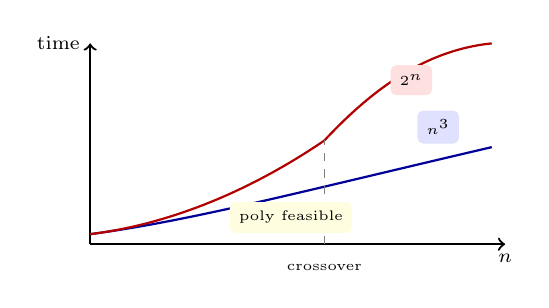
\begin{tikzpicture}[scale=0.85,every node/.style={font=\scriptsize}]
\draw[->,thick] (0,0)--(6.2,0) node[below] {$n$};
\draw[->,thick] (0,0)--(0,3.0) node[left] {time};
\draw[thick,blue!60!black] (0,0.15) .. controls (1.5,0.35) and (3.0,0.75) .. (6.0,1.45);
\node[font=\tiny,fill=blue!12,rounded corners=2pt] at (5.2,1.75) {$n^3$};
\draw[thick,red!70!black] (0,0.15) .. controls (1.2,0.30) and (2.4,0.80) .. (3.5,1.55) .. controls (4.2,2.30) and (5.0,2.90) .. (6.0,3.0);
\node[font=\tiny,fill=red!12,rounded corners=2pt] at (4.8,2.45) {$2^n$};
\draw[dashed,gray] (3.5,0)--(3.5,1.55);
\node[font=\tiny] at (3.5,-0.35) {crossover};
\node[font=\tiny,fill=yellow!12,rounded corners=2pt] at (3.0,0.40) {poly feasible};
\end{tikzpicture}
\caption{Polynomial $n^k$ vs.\ exponential $2^n$: beyond a modest $n$, exponential dominates regardless of constants; $P$ captures the feasible side.}
\label{fig:poly-vs-exp}
\end{figure}

\begin{example}[Problems in $P$]
$A_{DFA}$ is in $P$ ($O(n)$ simulation), $REACHABILITY$ ($s\to t$ in digraph) is in $P$ (BFS $O(n+m)$), $RELPRIME$ ($\gcd$) in $P$ (Euclid $O(\log n)$), and even linear programming is in $P$ (Khachiyan 1979). Edges $TIME$ depends on model but $P$ does not.
\end{example}

% ============================================================
\section{$NP$: Certificates and Nondeterminism}
\label{sec:NP}
\emph{Intuition:} a Sudoku is hard to solve but easy to \emph{check} given a filled board---the board is a certificate. $NP$ formalises ``checkable in polynomial time''.

\begin{definition}[Verifier view of $NP$]
A \emph{verifier} for $L$ is a DTM $V$ with $L=\{w\mid\exists c,\;|c|\le poly(|w|)\text{ and }V(w,c)=\text{accept}\}$ and $V$ runs in $poly(|w|)$ time. Then $NP=\{L\mid L\text{ has a poly-time verifier}\}$.
\end{definition}

\begin{definition}[NTM view of $NP$]
$NP=\{L\mid\exists\text{ NTM }N,\;L(N)=L,\;time_N(n)=O(n^k)\}$ for some $k$, where $time_N(n)$ is the height of the computation tree (longest branch). Branching is existential: $w\in L$ iff \emph{some} branch accepts within $n^k$ steps.
\end{definition}

\begin{theorem}[Equivalence of views]
Verifier $\iff$ NTM. Given verifier $V$, NTM guesses $c$ nondeterministically ($|c|\le n^k$ possibilities) then runs $V$; given NTM $N$, certificate is the sequence of nondeterministic choices leading to accept ($O(n^k)$ bits), verified by simulating $N$ deterministically along those choices.
\end{theorem}

\begin{example}[$NP$ examples]
$SAT=\{\langle\phi\rangle\mid\phi$ CNF satisfiable$\}$ is in $NP$: $c$ is assignment, $V$ checks clauses in $O(|\phi|)$. $CLIQUE=\{\langle G,k\rangle\mid G$ has $k$-clique$\}$ is in $NP$: $c$ is $k$-subset, $V$ checks all $\binom{k}{2}$ edges. $HAMPATH$ (Hamiltonian path) also in $NP$: $c$ is permutation, $V$ checks edges. All are believed not in $P$.
\end{example}

% TikZ 2: verifier vs NTM branching
\begin{figure}[h]
\centering
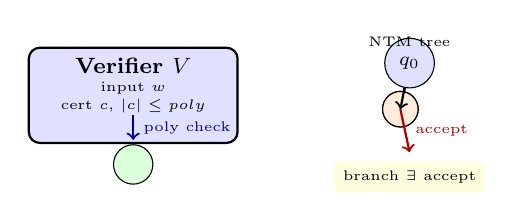
\begin{tikzpicture}[scale=0.78,every node/.style={font=\scriptsize}]
\begin{scope}
\draw[thick,fill=blue!12,rounded corners=4pt] (0,0) rectangle (3.4,1.55);
\node[font=\footnotesize\bfseries] at (1.7,1.25) {Verifier $V$};
\node[font=\tiny] at (1.7,0.90) {input $w$};
\node[font=\tiny] at (1.7,0.60) {cert $c$, $|c|\le poly$};
\draw[->,thick,blue!60!black] (1.7,0.45)--(1.7,0.05) node[midway,right,font=\tiny] {poly check};
\node[draw,fill=green!14,circle,minimum size=0.5cm] at (1.7, -0.35) {$\checkmark$};
\end{scope}
\begin{scope}[xshift=5.0cm]
\node[draw,circle,fill=blue!12,minimum size=0.6cm] (r) at (1.2,1.3) {$q_0$};
\foreach \a in {-0.9,-0.2,0.7} {\node[draw,circle,fill=orange!14,minimum size=0.45cm] at (0.15+ \a*0.0 +0.9,0.55) {}; \draw[->,thick] (r)--(0.15+0.9,0.55);}
\draw[->,thick,red!70!black] (0.15+0.9,0.55)--(1.2,-0.15) node[midway,right,font=\tiny] {accept};
\node[font=\tiny] at (1.2,1.65) {NTM tree};
\node[font=\tiny,fill=yellow!12,rounded corners=2pt] at (1.2,-0.55) {branch $\exists$ accept};
\end{scope}
\end{tikzpicture}
\caption{Two views of $NP$: poly-time verifier with short certificate vs.\ poly-time NTM with existential branching; they are equivalent via ``certificate = nondeterministic choices''.}
\label{fig:NP-views}
\end{figure}

Clearly $P\subseteq NP$ (take $c=\varepsilon$, or NTM is DTM). Whether $P=NP$ (can every checkable problem be solved feasibly?) is open and Clay Millennium.

% ============================================================
\section{Polynomial Reductions and $NP$-Completeness}
\label{sec:npc}
Reductions now must be \emph{polynomial-time} ($\le_p$), not just computable.

\begin{definition}[$\le_p$, $NP$-hard, $NP$-complete]
$A\le_p B$ if computable $f$ with $w\in A\iff f(w)\in B$ and $f$ runs in $poly(|w|)$ time (hence $|f(w)|\le poly(|w|)$). $B$ is \emph{$NP$-hard} if $\forall A\in NP,\;A\le_p B$. $B$ is \emph{$NP$-complete} if $B\in NP$ and $B$ is $NP$-hard. If any $NP$-complete $B$ is in $P$, then $P=NP$.
\end{definition}

% TikZ 3: NPC as hardest in NP
\begin{figure}[h]
\centering
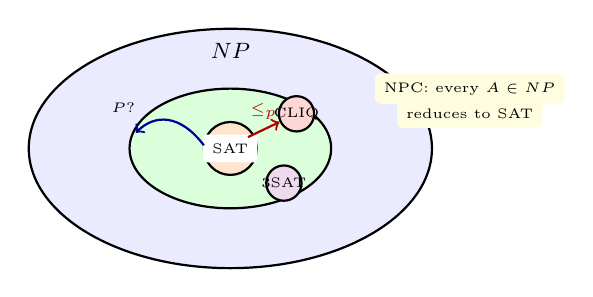
\begin{tikzpicture}[scale=0.80,every node/.style={font=\scriptsize}]
\draw[thick,fill=blue!8] (0,0) ellipse (3.2 and 1.9);
\draw[thick,fill=green!14] (0,0) ellipse (1.6 and 0.95);
\node[font=\footnotesize\bfseries] at (0,1.55) {$NP$};
\node[font=\tiny] at (-1.7,0.65) {$P$?};
\draw[thick,fill=orange!20] (0,0) circle (0.42);
\node[font=\tiny,fill=white,rounded corners=1pt] at (0,0) {SAT};
\draw[thick,fill=red!16] (1.05,0.55) circle (0.28); \node[font=\tiny] at (1.05,0.55) {CLIQ};
\draw[thick,fill=violet!14] (0.85,-0.55) circle (0.28); \node[font=\tiny] at (0.85,-0.55) {3SAT};
\draw[->,thick,blue!60!black] (-0.42,0.05) .. controls (-0.8,0.55) and (-1.2,0.55) .. (-1.5,0.25);
\node[font=\tiny,fill=yellow!12,rounded corners=2pt] at (3.8,0.95) {NPC: every $A\in NP$};
\node[font=\tiny,fill=yellow!12,rounded corners=2pt] at (3.8,0.55) {reduces to SAT};
\draw[->,thick,red!70!black] (0.28,0.18)--(0.78,0.42) node[midway,above,font=\tiny] {$\le_p$};
\end{tikzpicture}
\caption{$NP$-complete problems sit at the top of $NP$: every $NP$ language reduces to them in polynomial time; they stand or fall together for $P=NP$.}
\label{fig:npc-hardest}
\end{figure}

% ============================================================
\section{Cook--Levin Theorem: SAT is $NP$-Complete}
\label{sec:cook-levin}
\begin{theorem}[Cook 1971, Levin 1973]
$SAT$ (and $3SAT$ with $3$ literals per clause) is $NP$-complete.
\end{theorem}
\begin{proof}[Idea --- tableau]
Given NTM $N$ for $L\in NP$ running in $n^k$ time, on input $w$ build formula $\phi_{N,w}$ whose satisfying assignment encodes an accepting \emph{computation tableau} of $N$ on $w$: $n^k\times n^k$ grid of tape cells, head positions, and states over time. Variables $x_{i,j,s}$ mean ``cell $(i,j)$ at step $i$ holds symbol $s$''. Clauses enforce: (a) each cell has exactly one symbol, (b) initial row is $q_0w$, (c) each row follows from previous via $\delta$, (d) some row contains $q_{\rm accept}$. Construction is $O(n^{2k})$ time, poly in $|w|$, and $\phi_{N,w}$ satisfiable iff $N$ accepts $w$. Hence $L\le_p SAT$. Since $SAT\in NP$, $SAT$ is $NP$-complete; $3SAT$ follows by splitting long clauses with fresh variables (e.g.\ $(a_1\lor\cdots\lor a_k)\rightsquigarrow(a_1\lor a_2\lor z_1)\land(\overline{z_1}\lor a_3\lor z_2)\land\cdots$). \qed
\end{proof}

\begin{example}[Tableau size]
For $n=10$, $k=2$, tableau is $100\times100=10^4$ cells, each with $|\Gamma|+|Q|$ Boolean variables ($\approx20$), so $\approx2\times10^5$ variables and $O(n^{2k})$ clauses---polynomial but large; the theorem is existential, not practical. The clause-splitting for $3SAT$ adds $O(k)$ fresh $z$'s per long clause.
\end{example}

% ============================================================
\section{More $NP$-Complete Problems: CLIQUE}
\label{sec:clique}
We propagate completeness by chaining reductions.

\begin{theorem}[CLIQUE is $NP$-complete]
$3SAT\le_p CLIQUE$, so CLIQUE is $NP$-complete.
\end{theorem}
\begin{proof}[Sketch]
Given $3$CNF $\phi=C_1\land\cdots\land C_m$ with $C_i=(\ell_{i1}\lor\ell_{i2}\lor\ell_{i3})$, build graph $G$: $3m$ vertices $v_{i,j}$ labelled $\ell_{ij}$. Edge $v_{i,j}$--$v_{i',j'}$ iff $i\neq i'$ and labels not contradictory ($x$ vs.\ $\overline{x}$). Ask for $k=m$-clique. If $\phi$ satisfiable, pick one true literal per clause---its $m$ vertices are pairwise non-contradictory and cross-clause, so a clique; conversely, a $m$-clique picks one vertex per clause (clique cannot have two from same $C_i$ since intra-cluster non-edges), and its labels give a consistent assignment satisfying every clause. Map is $O(m^2)$ time. Since $3SAT$ is $NP$-complete, so is CLIQUE. \qed
\end{proof}

% Detail for intuition:
\begin{center}
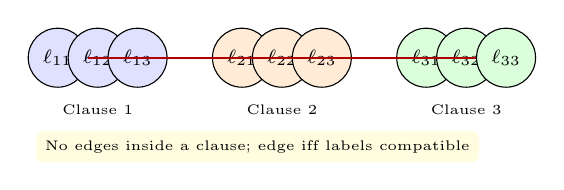
\begin{tikzpicture}[scale=0.78,every node/.style={font=\scriptsize}]
\foreach \i in {1,2,3} {\node[draw,circle,fill=blue!12,minimum size=0.55cm] (a\i) at (0.65*\i,1.1) {$\ell_{1\i}$};}
\foreach \i in {1,2,3} {\node[draw,circle,fill=orange!16,minimum size=0.55cm] (b\i) at (3.0+0.65*\i,1.1) {$\ell_{2\i}$};}
\foreach \i in {1,2,3} {\node[draw,circle,fill=green!14,minimum size=0.55cm] (c\i) at (6.0+0.65*\i,1.1) {$\ell_{3\i}$};}
\node[font=\tiny] at (1.3,0.25) {Clause 1}; \node[font=\tiny] at (4.3,0.25) {Clause 2}; \node[font=\tiny] at (7.3,0.25) {Clause 3};
\draw[thick,red!70!black] (a2)--(b1) (a2)--(b3) (a1)--(c1) (b2)--(c3);
\node[font=\tiny,fill=yellow!12,rounded corners=2pt] at (3.9,-0.35) {No edges inside a clause; edge iff labels compatible};
\end{tikzpicture}
\end{center}
If $\phi=(x\lor y\lor\overline{z})\land(\overline{x}\lor z\lor w)\land\cdots$, a $3$-clique touching each triangle corresponds to a satisfying choice.

% ============================================================
\section{Coping with $NP$-Completeness}
\label{sec:coping}
If $P\neq NP$, $NP$-complete problems have no polynomial algorithm. Practical coping:
\begin{itemize}[leftmargin=1.2em]
    \item \textbf{Approximation:} for optimisation (e.g.\ MIN-VERTEX-COVER within $2\times$ via maximal matching), trade optimality for poly time and prove ratio.
    \item \textbf{Fixed-parameter tractability (FPT):} $O(f(k)\,poly(n))$ for parameter $k$ (e.g.\ VERTEX-COVER $O(2^k n)$ when $k=$ cover size small). Kernelisation shrinks instance.
    \item \textbf{Heuristics \& solvers:} SAT solvers (CDCL), ILP, branch-and-bound exploit structure despite worst-case hardness; many real instances are easy.
    \item \textbf{Average case / random:} hardness is worst-case; random 3SAT has phase transition at clause/variable $\approx4.3$.
\end{itemize}
Recognising $NP$-completeness saves wasted effort on exact poly algorithms and directs you to the right compromise.

\begin{example}[Code: brute-force vs.\ verifier for CLIQUE]
\begin{lstlisting}[language=Python]
import itertools
def has_clique_bruteforce(G,k):
    for S in itertools.combinations(G.nodes, k):  # exponential
        if all(G.has_edge(u,v) for u,v in itertools.combinations(S,2)):
            return True
    return False
def verify_clique(G,k, cert):
    # cert = k nodes, verifier runs O(k^2)
    if len(cert)!=k or len(set(cert))!=k: return False
    return all(G.has_edge(u,v) for u,v in itertools.combinations(cert,2))
\end{lstlisting}
Brute force is $O(n^k)$; verifier is $O(k^2)$---the $P$ vs.\ $NP$ gap in code.
\end{example}

% ============================================================
\section{Chapter Notes}
Garey--Johnson is the $NP$-completeness catalogue; Arora--Barak gives modern treatment with PCP. Cook's original reduction used tableau; Karp (1972) listed 21 $NP$-complete problems including CLIQUE, HAMPATH, SUBSET-SUM. For $P$ vs.\ $NP$, see Fortnow's survey; relativisation and natural proofs explain why simple diagonalisation fails, motivating circuit and proof complexity approaches.

% ============================================================
\section{Exercises}
\label{sec:ch08-exercises}
\begin{enumerate}[label=E8.\arabic*, leftmargin=*, itemsep=0.8em]
\item \textbf{Verifier vs.\ NTM.} Give verifier for $HAMPATH$ and convert to NTM: certificate is permutation of $n$ vertices, verifier checks each consecutive pair is an edge in $O(n^2)$. Count certificate bits $O(n\log n)$.
\item \textbf{Cook--Levin size.} For NTM with $|\Gamma|=3$, $|Q|=10$, $t(n)=n^2$, bound variables and clauses in $\phi_{N,w}$ as polynomials in $n$; why does poly size matter for $\le_p$?
\item \textbf{$SAT\to3SAT$.} Reduce clause $(x_1\lor x_2\lor x_3\lor x_4)$ to two $3$-clauses with fresh $z$: $(x_1\lor x_2\lor z)\land(\overline{z}\lor x_3\lor x_4)$; prove equisatisfiable and generalise to $k$-clauses with $k-3$ fresh variables.
\item \textbf{CLIQUE reduction trace.} For $\phi=(x\lor y\lor\overline{z})\land(\overline{x}\lor z\lor w)$, build $G$ with $9$ vertices (3 per clause), list edges, exhibit $2$-clique vs.\ $3$-clique and read off satisfying assignment $x=1,y=0,\dots$; show unsatisfiable $\phi$ yields no $3$-clique.
\item \textbf{Coping.} Show $2$-approximation for MIN-VERTEX-COVER: take maximal matching $M$, return endpoints of $M$; prove $|M|\le OPT\le2|M|$ and $O(n+m)$ time. Why does this not imply $P=NP$?
\end{enumerate}
% End of Chapter 8
